\chapter[Preliminares ]{Preliminares }\label{ch:capitulo3}
En este capítulo presentaremos diversos términos fundamentales. El objetivo principal es entregar un marco teórico sobre los conceptos que se utilizan en los siguientes capítulos para definir las técnicas utilizadas.
\begin{definition}[Celdas]
\label{def:cel}
Una celda consiste en una porción que mide 8 pixeles de alto por 8 pixeles de ancho.
\end{definition}
\begin{definition}[Bloques]
\label{def:blo}
Un bloque es una porción de la imagen que corresponde a 2x2 celdas.
\end{definition}
\begin{definition}[Bins]
\label{def:bin}
No se como explicarlo, need halp ! :(
\end{definition}

\section{Histogram of Oriented Gradients}\label{subsec:hog}
\textit{Histogram of Oriented Gradients (HOG)} presentado por Dalal y Triggs~\cite{hog2005}, es un descriptor de características utilizado en visión por computador y procesamiento de imágenes, Este algoritmo sirve para representar objetos (latas, botellas, autos, personas, rostros, etc). En términos generales, HOG, es una técnica que cuenta las ocurrencias de las orientaciones de los gradiente en partes especificas de una imagen. Este método calcula un espacio de celdas superpuestas con el fin de normalizar las muestras locales y aumentar la precisión.

HOG cuenta con ciertos pasos que se deben realizar para obtener el descriptor de una imagen, esto se puede ver en la Figura~\ref{fig:hog_procedure} y a continuación se detallan las etapas que componen el algoritmo HOG.
\begin{figure}[tb]
  \centering
   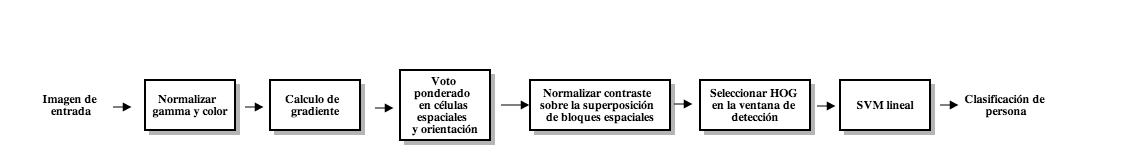
\includegraphics[width=1\textwidth]{Figuras/hog-procedure.png}
   \caption{Procedimiento de HOG}
   \label{fig:hog_procedure}
\end{figure}

\subsection{Procedimiento de HOG}
Felzenszwalb et al.~\cite{Felzenszwalb2010}, dividen la imagen en celdas (ver Definición~\ref{def:cel}), sin superposición. Luego, por cada pixel dentro de una celda se acumulan los histogramas de orientación de gradientes. Estos histogramas capturan propiedades de forma local dentro de la celda. a su vez, estos histogramas son invariantes a pequeñas deformaciones.
El gradiente en cada pixel está discretizado en uno de los nueve contenedores(\textit{bins}) de orientación, y cada pixel vota por la orientación de su gradiente, con un valor que depende de la magnitud del gradiente. Para las imágenes en color, se calcula el gradiente de cada canal de color, eligiendo el canal con la mayor cantidad de pixeles donde la magnitud del gradiente esa mayor.

En la Figura~\ref{fig:blocks_cells} se puede apreciar la división de los bloques y las celdas antes descritas.

\begin{figure}[tb]
  \centering
   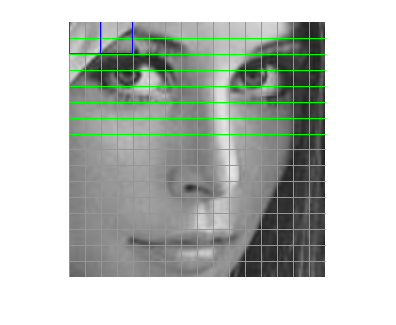
\includegraphics[width=0.5\textwidth]{Figuras/lena-grid.png}
   \caption{Bloque 1 (azul), bloque 2 (rojo), celdas (verde)}
   \label{fig:blocks_cells}
\end{figure}

Finalmente, cada histograma de las celdas es normalizado con respecto a la energía del gradiente en un vecindario al rededor de la celda. Se observan los cuatro bloques de 2x2 de celdas que contienen una celda particular y luego se normaliza el histograma cada celda dada con respecto a la energía total en cada uno de estos bloques. Esto entrega un vector de longitud 9x4 que representa la información local de gradiente dentro de una célula.
\section{Pirámide}\label{sec:pyra}
La pirámide, consiste en hacer varias iteraciones de una misma imagen con distintas resoluciones, donde en cada nivel de resolución se extraen las características más representativas con el descriptor de HOG. La Figura~\ref{fig:hog_pyra}, muestra los histogramas obtenidos luego de pasar una imagen por tres niveles de la pirámide, estos niveles son representados por $\lambda$ y en la fase de entrenamiento tienen un valor de 5, es decir, cinco niveles de profundidad.

\begin{figure}[tb]
  \centering
   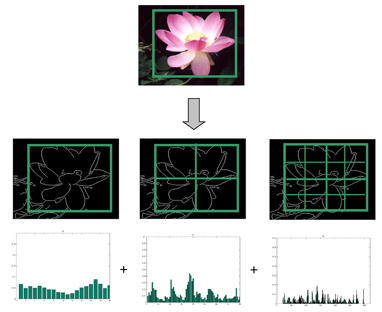
\includegraphics[width=1\textwidth]{Figuras/phog.jpg}
   \caption{Pirámide de HOG~\cite{pyra}}
   \label{fig:hog_pyra}
\end{figure}

\section{Filtro y score}\label{sec:fas}


\section{SVM}\label{sec:svm}


\section{Resumen}\label{sec:resumen}

